\documentclass[helvetica]{seminar} 
\input{xy}
\xyoption{all}
\usepackage{graphicx} 
\usepackage{slidesec} 
% \usepackage{url}
\usepackage{hyperref}
\usepackage[framemethod=TikZ]{mdframed}
\usepackage{color}
\usepackage[normalem]{ulem}  

\def\dash---{\unskip\kern.16667em---\penalty\exhyphenpenalty\hskip.16667em\ignorespaces}
\long\def\symbolfootnote[#1]#2{\begingroup%
\def\thefootnote{\fnsymbol{footnote}}\footnote[#1]{#2}\endgroup}

% to fix problems making landscape seminar pdfs
% Letter...
\pdfpagewidth=11truein
\pdfpageheight=8.5truein
\pdfhorigin=1truein     % default value(?), but doesn't work without
\pdfvorigin=1truein     % default value(?), but doesn't work without
% A4
%\pdfpagewidth=297truemm % your milage may vary....
%\pdfpageheight=210truemm
%\pdfhorigin=1truein     % default value(?), but doesn't work without
%\pdfvorigin=1truein     % default value(?), but doesn't work without


\renewcommand{\familydefault}{\sfdefault}  
 
\input{seminar.bug} 
\input{seminar.bg2} % See the Seminar bugs list 
 
\slideframe{none} 
 
 
\usepackage{fancyhdr} 
 
% Headers and footers personalization using the `fancyhdr' package 
\fancyhf{} % Clear all fields 
\renewcommand{\headrulewidth}{0mm} 
\renewcommand{\footrulewidth}{0.1mm} 
 
\fancyfoot[L]{\tiny IETF 98} 
\fancyfoot[C]{\tiny IASA 2.0}
\fancyfoot[R]{\tiny \theslide} 
 
 
% To center horizontally the headers and footers (see seminar.bug) 
\renewcommand{\headwidth}{\textwidth} 

% To adjust the frame length to the header and footer ones 
\autoslidemarginstrue 
\pagestyle{fancy} 
 

\newcommand{\heading}[1]{% 
  \begin{center} 
    \large\bf 
    #1 
  \end{center} 
  \vspace{.4 in}} 



\begin{document}

\begin{slide}
\begin{center}
\vspace{.5 in}
\LARGE{{\bf}Report from IASA 2.0 Virtual Workshops\\{\small \verb^draft-hall-iasa20-workshops-report-00^}}\\
\vspace{.2in}
\large{
\begin{tabular}{ c c }
Joseph Lorenzo Hall & A. Jean Mahoney\\
CDT & \\
\url{joe@cdt.org} & \url{mahoney@nostrum.com}
\end{tabular}
}
\end{center}
\end{slide}

\centerslidesfalse 

\begin{slide}
\heading{Outline}

%\vspace{-8ex}         %for long lists
\begin{itemize}
\item Terminology and Organizational Structure
\item Issues Raised (listed in order of perceived importance):
  \begin{itemize}
  \item Structural and Organizational Issues
  \item Funding Issues
  \item Transparency and Communication Issues
  \item Staff and Volunteer Resource Issues
  \item Internal IAOC Organizational Issues
  \end{itemize}
\end{itemize}

\end{slide}

\begin{slide}

\heading{Terminology}

{\footnotesize
\begin{itemize}
\item \textbf{IASA:} ``IETF Administrative Support Activity'' - An
  organized activity that provides administrative support for the
  IETF, the IAB and the IESG.
\item \textbf{IAOC:} ``IETF Administrative Oversight Committee'' - A
  largely IETF-selected committee that oversees and directs
  IASA. Accountable to the IETF community.
\item \textbf{IAD:} ``IETF Administrative Director'' - The sole staff
  member responsible for carrying out the work of the IASA. An ISOC
  employee.
\item \textbf{IETF Trust:} Acquires, maintains, and licenses
  intellectual and other property used in connection with the
  administration of the IETF. Same composition as IAOC.
\end{itemize}
}

\end{slide}


\begin{slide}

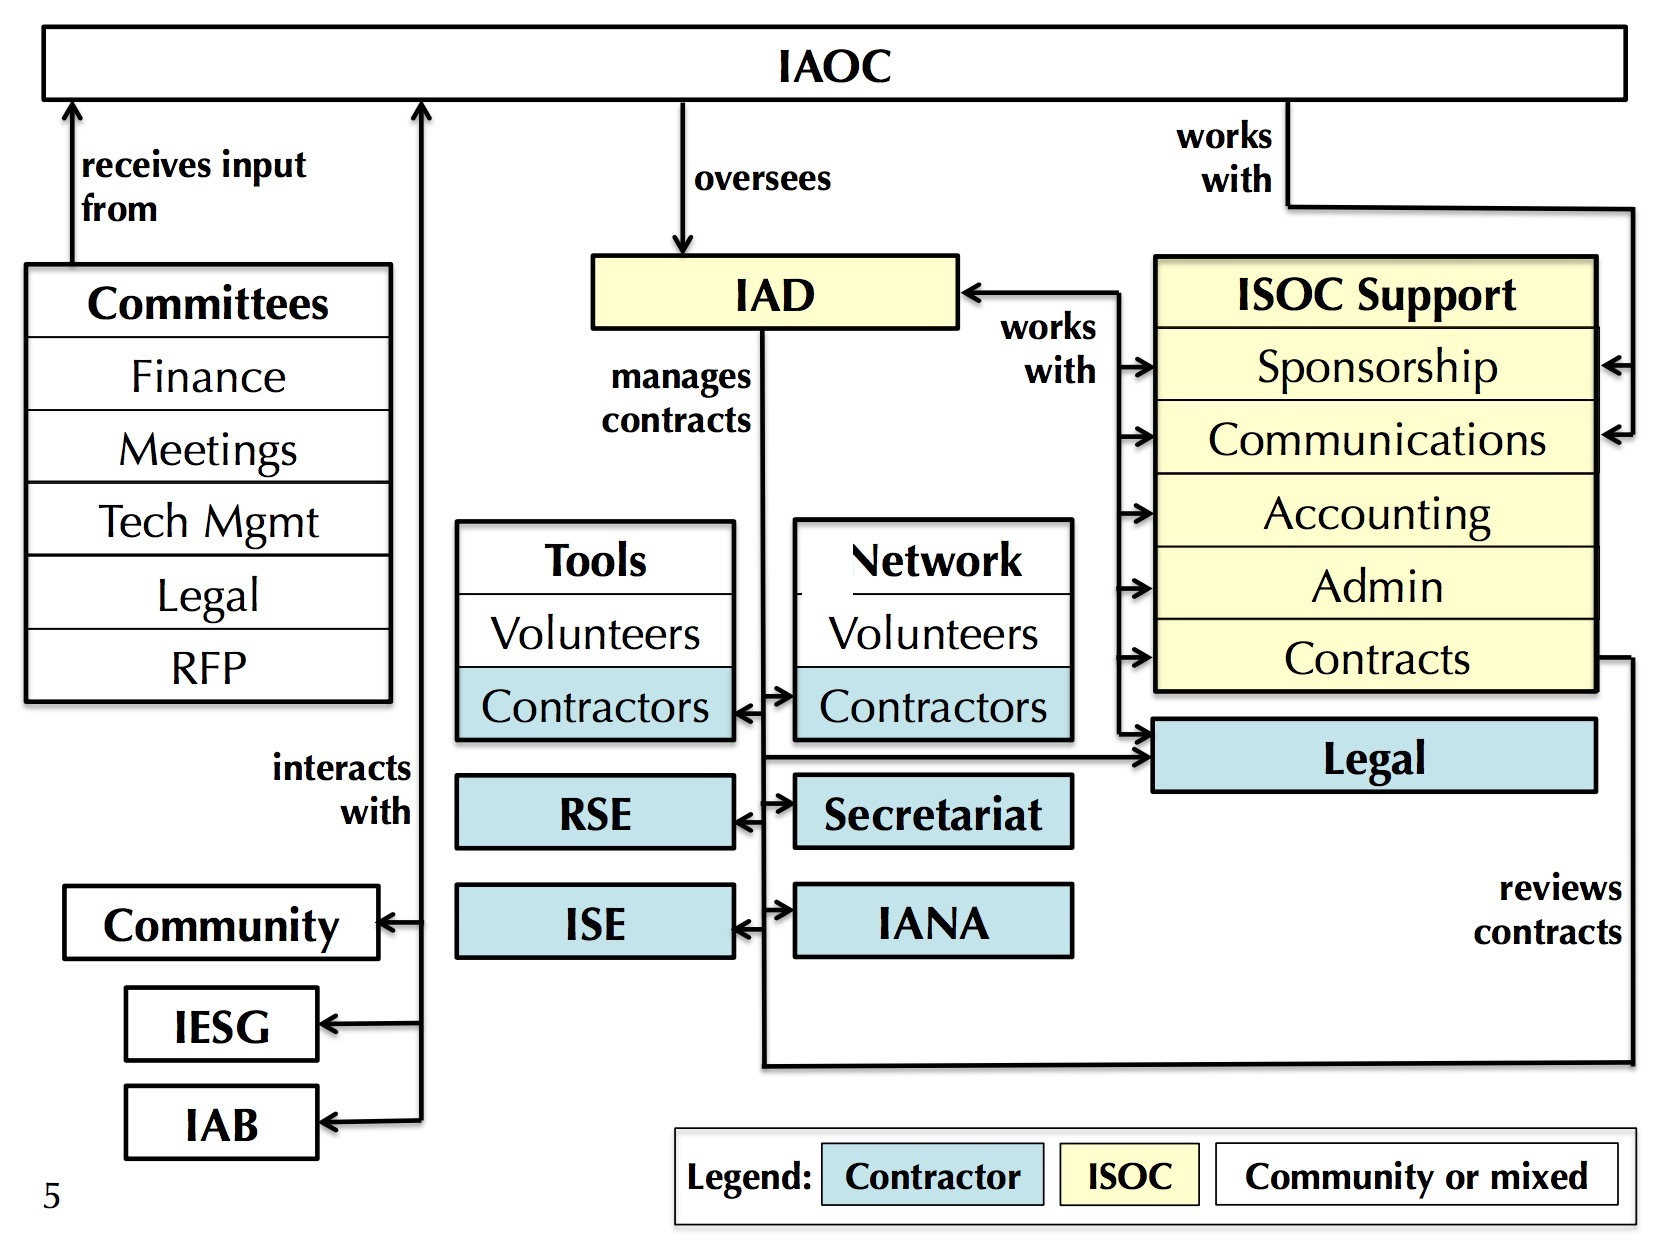
\includegraphics[width=4.0in]{IASA-org-chart}

\end{slide}

\begin{slide}
\heading{Structural and Organizational Issues}

Workshop chairs identified structural and organizational issues:
{\footnotesize
\begin{itemize}
\item The \textbf{line between the IETF and ISOC is not
  organizationally clear-cut}, which has led to issues around
  transparency, allocation of staff time and priorities, budgeting,
  and clarity of who is responsible for what.
\item The \textbf{respective roles of ISOC, the IETF chair, the IAOC,
  and the secretariat} in representing the IETF to sponsors and donors
  and communicating with them \textbf{are not clear}.
\item Having ISOC represent the IETF to sponsors and donors:
  \begin{itemize}
  \item \textbf{creates confusion} about why the IETF does not
    represent itself,
  \item yields questions about why ISOC does not instead increase its
    IETF support and \textbf{how donations can be guaranteed to be
      dedicated to the IETF}, and
  \item can result in \textbf{those soliciting sponsorships and
    donations having a lack of familiarity with IETF work}.
  \end{itemize}
\end{itemize}
}

\end{slide}

\begin{slide}
\heading{Structural and Organizational Issues}

Structural/Organizational issues raised in the IASA virtual workshops:
\begin{itemize}
\item Delineation of roles/branding
\item Control and policy authority
\item Accounting structure
\item Benefits of lack of rigid formality
\end{itemize}

\end{slide}


\begin{slide}
\heading{Funding Issues}

Workshop chairs identified funding issues:
{\footnotesize
\begin{itemize}
\item \textbf{Meeting fees are currently an important source of
  revenue}, but remote participation and other factors may be
  responsible for \textbf{declining in-person meeting attendance going
    forward}.  Even if fees were charged for remote participation,
  charging the same for remote and in-person attendance is unlikely to
  be a viable way to make up the difference.
\item While there has been a lot of \textbf{sponsor support} for,
  e.g., meeting hosting, getting support for the full sponsorship
  program is not easy.  The value to sponsors is not always obvious,
  the IETF community is sometimes critical or unappreciative, and the
  same sponsors get tapped again and again for many related but
  different opportunities.
\item \textbf{Relying heavily on meeting-based revenue is somewhat at
  odds} with the fact that much of the IETF's work takes place outside
  of in-person meetings.
\item The \textbf{IETF is increasingly relying on professional
  services} to support its activities, causing expenses to grow.
\end{itemize}
}

\end{slide}

\begin{slide}
\heading{Funding Issues}

Funding issues raised in the IASA virtual workshops:
\begin{itemize}
\item Relevant draft: \href{https://tools.ietf.org/html/draft-arkko-ietf-finance-thoughts-00}{I-D.arkko-ietf-finance-thoughts}
\item Funding as a measure of IETF relevance
\item Importance of having multiple funding streams
\item Is the current mix optimal? What would be better?
\item Is it still true that a major function of ISOC is to make up
  shortfalls?
\item Can we look to other open source sponsorship funding models?
\item Sponsorship is far more cumbersome than simply finding funds.
\item How is funding outreach done?
\end{itemize}

\end{slide}


\begin{slide}
\heading{Transparency and Communication Issues}

Workshop chairs identified transparency/communication issues:
{\footnotesize
\begin{itemize}
\item \textbf{IAOC has typically been perceived to operate less
  transparently} than what is the norm for IETF processes and other
  IETF leadership bodies.
\item \textbf{Lack of transparency has some roots} in concerns about
  confidentiality of contract terms and business relationships, and
  fear of community reaction to administrative decisions.
\item \textbf{Requirements} from the community about IAOC transparency
  expectations \textbf{are not clear}.
\end{itemize}
}

\end{slide}

\begin{slide}
\heading{Transparency and Communication Issues}

Transparency/Communications issues raised in the IASA virtual
workshops:
{\footnotesize
\begin{itemize}
\item IAOC and IASA could better communicate with the IETF community
  \begin{itemize}
  \item Should the IETF community document the transparency
    requirement clearly? (e.g., set the default to be open and publish
    an exception list for confidential or sensitive matters.)
  \item What is behind lack of transparency outside of
    proprietary/confidentiality concerns? (FONMO: fear of not missing
    out? lack of desire to rehash previous complex discussions?)
  \end{itemize}
\item Need to balance community impatience with administrivia and
  their desire to provide input
  \begin{itemize}
  \item Boring details ``which are boring until they're not, and then
    everyone is surprised.''
  \item Can IETF community get insight into what the IAOC is going to
    do, as opposed to what it has just done?
  \end{itemize}
\end{itemize}
}
  
\end{slide}


\begin{slide}
\heading{Staff and Volunteer Resource Issues}

Workshop chairs identified staff/volunteer resource issues:
{\footnotesize
\begin{itemize}
\item \textbf{IAD workload is (much) more than a full-time job}, but
  we have one staff person allocated to it.
\item IASA tasks touch on a wider variety of topics and
  \textbf{require more different kinds of expertise than 10 years ago}
  (visa issues, local social/political/health issues, new modes of
  fundraising, etc.), but the job descriptions and skill sets of staff
  and volunteers do not always match these needs.
\item \textbf{Very few community members have the time, support, and
  interest to stand for the IAOC} (or even participate in
  administrative discussions, unless something goes astray), and many
  who do are self-funding their work.
\end{itemize}
}

\end{slide}

\begin{slide}
\heading{Staff and Volunteer Resource Issues}

Staff/Volunteer issues raised in the IASA virtual workshops:
\begin{itemize}
\item Do we understand the scope and authority for each committee?
  E.g., if a committee can make a decision that is easily overturned
  by the IAOC, that seems like a mismatch.
\item It would be helpful to better define roles of individuals on
  committees and how they are chosen. E.g., what must be done by paid
  contractors?
\item It all seems rather organically complex but not necessarily in a
  directed fasion (would it look like this if we consciously
  designed?)
\end{itemize}

\end{slide}


\begin{slide}
\heading{Internal IAOC Organizational Issues}

Workshop chairs identified internal IAOC organizational issues:
{\footnotesize
\begin{itemize}
\item \textbf{IAOC has constrained membership:} The IAOC has 4 ex
  officio members (IETF Chair, IAB Chair, ISOC CEO, IAD (non-voting)),
  and 5 appointed members.  One of 5 members is appointed by the ISOC
  Board of Trustees, and is traditionally expected not to stand for
  IAOC Chair.  This yields:
  \begin{itemize}
  \item A small pool from which to select the IAOC Chair/IETF Trust
    Chair
  \item Two "worker bees" for IAOC (after appointing IAOC/IETF Trust
    Chairs)
  \end{itemize}
\item \textbf{Requiring that the IAOC and the IETF Trust be
  constituted by the same group of people overloads the job
  responsibilities of both roles}, narrows the pool of individuals
  willing and able to serve on the IAOC, and creates the potential for
  conflicts in cases where the creation of Trust policies requires
  IAOC oversight.
\item \textbf{Requiring that the IAB chair serve on the IAOC overloads
  the IAB Chair's job responsibilities} and narrows the pool of people
  willing and able to serve as IAB Chair.  The same may be true for
  the IETF Chair.
\end{itemize}
}

\end{slide}

\begin{slide}
\heading{Internal IAOC Organizational Issues}

IAOC organizational issues raised in the IASA virtual workshops:
\begin{itemize}
\item Populating the IAOC is difficult because is there are so many
  leadership positions. What does a future IAOC need to look like?
  \begin{itemize}
  \item Seems to be pretty clear that the IAOC needs to be bigger, and
    needs to have more general members.
  \item Relying on volunteers for the IAOC's large volume of work may
    be unreasonable
  \end{itemize}
\item To the extend IAOC provides an oversight function, it is very
  thin in current composition
\item It seems no longer ``convenient'' that the IAOC and Trust are
  heavily overlapping boddies
\end{itemize}

\end{slide}




\end{document} 

                
